% Neural network diagram
% Made with Xematics. Positions are in px (1 px = 0.75 pt), as in the SVG export.
\documentclass[tikz, border=4pt]{standalone}
\usepackage[T1]{fontenc}
\usepackage{lmodern}
\definecolor{xm1}{HTML}{FFFFFF}
\definecolor{xm2}{HTML}{F1F2F4}
\definecolor{xm3}{HTML}{4B5563}
\definecolor{xm4}{HTML}{FBE8C4}
\definecolor{xm5}{HTML}{B97800}
\definecolor{xm6}{HTML}{B8C0CC}
\definecolor{xm7}{HTML}{D4E8F5}
\definecolor{xm8}{HTML}{0072B2}
\definecolor{xm9}{HTML}{DFE3E8}
\definecolor{xm10}{HTML}{AEB3B9}
\definecolor{xm11}{HTML}{6B7280}
\definecolor{xm12}{HTML}{1F2937}
\begin{document}
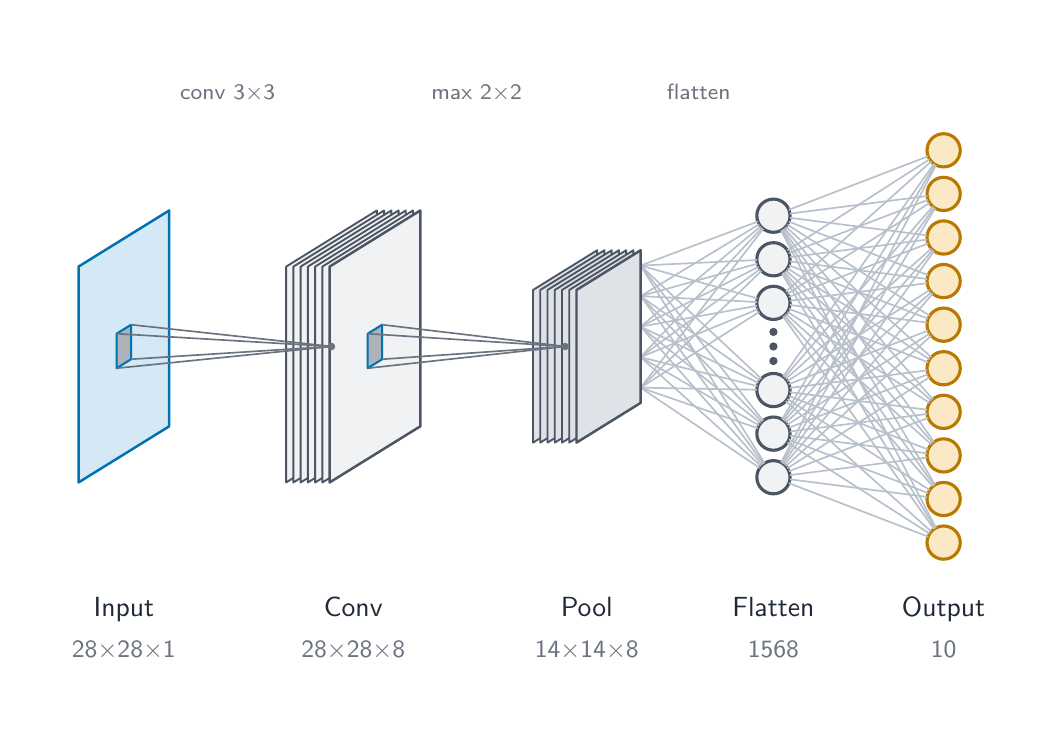
\begin{tikzpicture}[x=0.75pt, y=-0.75pt]
  \tikzset{
    xm hidden/.style={circle, minimum size=12pt, inner sep=0, outer sep=0, fill=xm2, draw=xm3, line width=1.13pt},
    xm output/.style={circle, minimum size=12pt, inner sep=0, outer sep=0, fill=xm4, draw=xm5, line width=1.13pt},
    xm edge/.style={draw=xm6, line width=0.6pt},
    xm map input/.style={fill=xm7, draw=xm8, line width=0.9pt, line join=round},
    xm map hidden back/.style={fill=xm2, draw=xm3, line width=0.68pt, line join=round},
    xm map hidden/.style={fill=xm2, draw=xm3, line width=0.9pt, line join=round},
    xm map pool back/.style={fill=xm9, draw=xm3, line width=0.68pt, line join=round},
    xm map pool/.style={fill=xm9, draw=xm3, line width=0.9pt, line join=round},
    xm dots/.style={fill=xm3},
    xm window/.style={fill=xm10, draw=xm8, line width=0.75pt, line join=round},
    xm ray/.style={draw=xm11, line width=0.6pt},
    xm ray end/.style={fill=xm11},
    xm name xm12/.style={text=xm12, inner sep=0, font=\sffamily\fontsize{9.75}{11.7}\selectfont},
    xm size xm11/.style={text=xm11, inner sep=0, font=\sffamily\fontsize{9}{10.8}\selectfont},
    xm op xm11/.style={text=xm11, inner sep=0, font=\sffamily\fontsize{8.25}{9.9}\selectfont},
  }
  \fill[xm1] (0,0) rectangle (484.65,329.25);
  % Neurons
  \node[xm hidden] (n-3-0) at (359.3,90.59) {};
  \node[xm hidden] (n-3-1) at (359.3,111.59) {};
  \node[xm hidden] (n-3-2) at (359.3,132.59) {};
  \node[xm hidden] (n-3-1565) at (359.3,174.59) {};
  \node[xm hidden] (n-3-1566) at (359.3,195.59) {};
  \node[xm hidden] (n-3-1567) at (359.3,216.59) {};
  \node[xm output] (n-4-0) at (441.3,59.09) {};
  \node[xm output] (n-4-1) at (441.3,80.09) {};
  \node[xm output] (n-4-2) at (441.3,101.09) {};
  \node[xm output] (n-4-3) at (441.3,122.09) {};
  \node[xm output] (n-4-4) at (441.3,143.09) {};
  \node[xm output] (n-4-5) at (441.3,164.09) {};
  \node[xm output] (n-4-6) at (441.3,185.09) {};
  \node[xm output] (n-4-7) at (441.3,206.09) {};
  \node[xm output] (n-4-8) at (441.3,227.09) {};
  \node[xm output] (n-4-9) at (441.3,248.09) {};
  % Connections 2
  \draw[xm edge] (295.3,114.62) -- (n-3-0);
  \draw[xm edge] (295.3,114.62) -- (n-3-1);
  \draw[xm edge] (295.3,114.62) -- (n-3-2);
  \draw[xm edge] (295.3,114.62) -- (n-3-1565);
  \draw[xm edge] (295.3,114.62) -- (n-3-1566);
  \draw[xm edge] (295.3,114.62) -- (n-3-1567);
  \draw[xm edge] (295.3,129.33) -- (n-3-0);
  \draw[xm edge] (295.3,129.33) -- (n-3-1);
  \draw[xm edge] (295.3,129.33) -- (n-3-2);
  \draw[xm edge] (295.3,129.33) -- (n-3-1565);
  \draw[xm edge] (295.3,129.33) -- (n-3-1566);
  \draw[xm edge] (295.3,129.33) -- (n-3-1567);
  \draw[xm edge] (295.3,144.03) -- (n-3-0);
  \draw[xm edge] (295.3,144.03) -- (n-3-1);
  \draw[xm edge] (295.3,144.03) -- (n-3-2);
  \draw[xm edge] (295.3,144.03) -- (n-3-1565);
  \draw[xm edge] (295.3,144.03) -- (n-3-1566);
  \draw[xm edge] (295.3,144.03) -- (n-3-1567);
  \draw[xm edge] (295.3,158.74) -- (n-3-0);
  \draw[xm edge] (295.3,158.74) -- (n-3-1);
  \draw[xm edge] (295.3,158.74) -- (n-3-2);
  \draw[xm edge] (295.3,158.74) -- (n-3-1565);
  \draw[xm edge] (295.3,158.74) -- (n-3-1566);
  \draw[xm edge] (295.3,158.74) -- (n-3-1567);
  \draw[xm edge] (295.3,173.45) -- (n-3-0);
  \draw[xm edge] (295.3,173.45) -- (n-3-1);
  \draw[xm edge] (295.3,173.45) -- (n-3-2);
  \draw[xm edge] (295.3,173.45) -- (n-3-1565);
  \draw[xm edge] (295.3,173.45) -- (n-3-1566);
  \draw[xm edge] (295.3,173.45) -- (n-3-1567);
  % Connections 3
  \draw[xm edge] (n-3-0) -- (n-4-0);
  \draw[xm edge] (n-3-0) -- (n-4-1);
  \draw[xm edge] (n-3-0) -- (n-4-2);
  \draw[xm edge] (n-3-0) -- (n-4-3);
  \draw[xm edge] (n-3-0) -- (n-4-4);
  \draw[xm edge] (n-3-0) -- (n-4-5);
  \draw[xm edge] (n-3-0) -- (n-4-6);
  \draw[xm edge] (n-3-0) -- (n-4-7);
  \draw[xm edge] (n-3-0) -- (n-4-8);
  \draw[xm edge] (n-3-0) -- (n-4-9);
  \draw[xm edge] (n-3-1) -- (n-4-0);
  \draw[xm edge] (n-3-1) -- (n-4-1);
  \draw[xm edge] (n-3-1) -- (n-4-2);
  \draw[xm edge] (n-3-1) -- (n-4-3);
  \draw[xm edge] (n-3-1) -- (n-4-4);
  \draw[xm edge] (n-3-1) -- (n-4-5);
  \draw[xm edge] (n-3-1) -- (n-4-6);
  \draw[xm edge] (n-3-1) -- (n-4-7);
  \draw[xm edge] (n-3-1) -- (n-4-8);
  \draw[xm edge] (n-3-1) -- (n-4-9);
  \draw[xm edge] (n-3-2) -- (n-4-0);
  \draw[xm edge] (n-3-2) -- (n-4-1);
  \draw[xm edge] (n-3-2) -- (n-4-2);
  \draw[xm edge] (n-3-2) -- (n-4-3);
  \draw[xm edge] (n-3-2) -- (n-4-4);
  \draw[xm edge] (n-3-2) -- (n-4-5);
  \draw[xm edge] (n-3-2) -- (n-4-6);
  \draw[xm edge] (n-3-2) -- (n-4-7);
  \draw[xm edge] (n-3-2) -- (n-4-8);
  \draw[xm edge] (n-3-2) -- (n-4-9);
  \draw[xm edge] (n-3-1565) -- (n-4-0);
  \draw[xm edge] (n-3-1565) -- (n-4-1);
  \draw[xm edge] (n-3-1565) -- (n-4-2);
  \draw[xm edge] (n-3-1565) -- (n-4-3);
  \draw[xm edge] (n-3-1565) -- (n-4-4);
  \draw[xm edge] (n-3-1565) -- (n-4-5);
  \draw[xm edge] (n-3-1565) -- (n-4-6);
  \draw[xm edge] (n-3-1565) -- (n-4-7);
  \draw[xm edge] (n-3-1565) -- (n-4-8);
  \draw[xm edge] (n-3-1565) -- (n-4-9);
  \draw[xm edge] (n-3-1566) -- (n-4-0);
  \draw[xm edge] (n-3-1566) -- (n-4-1);
  \draw[xm edge] (n-3-1566) -- (n-4-2);
  \draw[xm edge] (n-3-1566) -- (n-4-3);
  \draw[xm edge] (n-3-1566) -- (n-4-4);
  \draw[xm edge] (n-3-1566) -- (n-4-5);
  \draw[xm edge] (n-3-1566) -- (n-4-6);
  \draw[xm edge] (n-3-1566) -- (n-4-7);
  \draw[xm edge] (n-3-1566) -- (n-4-8);
  \draw[xm edge] (n-3-1566) -- (n-4-9);
  \draw[xm edge] (n-3-1567) -- (n-4-0);
  \draw[xm edge] (n-3-1567) -- (n-4-1);
  \draw[xm edge] (n-3-1567) -- (n-4-2);
  \draw[xm edge] (n-3-1567) -- (n-4-3);
  \draw[xm edge] (n-3-1567) -- (n-4-4);
  \draw[xm edge] (n-3-1567) -- (n-4-5);
  \draw[xm edge] (n-3-1567) -- (n-4-6);
  \draw[xm edge] (n-3-1567) -- (n-4-7);
  \draw[xm edge] (n-3-1567) -- (n-4-8);
  \draw[xm edge] (n-3-1567) -- (n-4-9);
  % Layers
  \draw[xm map input] (24.5,115.11) -- (68.18,88.07) -- (68.18,192.07) -- (24.5,219.11) -- cycle;
  \draw[xm map hidden back] (124.54,115.11) -- (168.22,88.07) -- (168.22,192.07) -- (124.54,219.11) -- cycle;
  \draw[xm map hidden back] (128.03,115.11) -- (171.71,88.07) -- (171.71,192.07) -- (128.03,219.11) -- cycle;
  \draw[xm map hidden back] (131.52,115.11) -- (175.2,88.07) -- (175.2,192.07) -- (131.52,219.11) -- cycle;
  \draw[xm map hidden back] (135.01,115.11) -- (178.69,88.07) -- (178.69,192.07) -- (135.01,219.11) -- cycle;
  \draw[xm map hidden back] (138.5,115.11) -- (182.18,88.07) -- (182.18,192.07) -- (138.5,219.11) -- cycle;
  \draw[xm map hidden back] (141.99,115.11) -- (185.67,88.07) -- (185.67,192.07) -- (141.99,219.11) -- cycle;
  \draw[xm map hidden] (145.48,115.11) -- (189.16,88.07) -- (189.16,192.07) -- (145.48,219.11) -- cycle;
  \draw[xm map pool back] (243.48,126.38) -- (274.36,107.26) -- (274.36,180.8) -- (243.48,199.92) -- cycle;
  \draw[xm map pool back] (246.97,126.38) -- (277.85,107.26) -- (277.85,180.8) -- (246.97,199.92) -- cycle;
  \draw[xm map pool back] (250.46,126.38) -- (281.34,107.26) -- (281.34,180.8) -- (250.46,199.92) -- cycle;
  \draw[xm map pool back] (253.95,126.38) -- (284.83,107.26) -- (284.83,180.8) -- (253.95,199.92) -- cycle;
  \draw[xm map pool back] (257.44,126.38) -- (288.32,107.26) -- (288.32,180.8) -- (257.44,199.92) -- cycle;
  \draw[xm map pool back] (260.93,126.38) -- (291.81,107.26) -- (291.81,180.8) -- (260.93,199.92) -- cycle;
  \draw[xm map pool] (264.42,126.38) -- (295.3,107.26) -- (295.3,180.8) -- (264.42,199.92) -- cycle;
  \fill[xm dots] (359.3,146.59) circle[radius=2];
  \fill[xm dots] (359.3,153.59) circle[radius=2];
  \fill[xm dots] (359.3,160.59) circle[radius=2];
  \draw[xm window] (42.84,147.44) -- (49.83,143.11) -- (49.83,159.75) -- (42.84,164.08) -- cycle;
  \draw[xm ray] (42.84,147.44) -- (146.38,153.59);
  \draw[xm ray] (49.83,143.11) -- (146.38,153.59);
  \draw[xm ray] (49.83,159.75) -- (146.38,153.59);
  \draw[xm ray] (42.84,164.08) -- (146.38,153.59);
  \fill[xm ray end] (146.38,153.59) circle[radius=1.8];
  \draw[xm window] (163.82,147.44) -- (170.81,143.11) -- (170.81,159.75) -- (163.82,164.08) -- cycle;
  \draw[xm ray] (163.82,147.44) -- (258.92,153.59);
  \draw[xm ray] (170.81,143.11) -- (258.92,153.59);
  \draw[xm ray] (170.81,159.75) -- (258.92,153.59);
  \draw[xm ray] (163.82,164.08) -- (258.92,153.59);
  \fill[xm ray end] (258.92,153.59) circle[radius=1.8];
  % Labels
  \node[xm name xm12, anchor=base] at (46.34,283.84) {Input};
  \node[xm size xm11, anchor=base] at (46.34,303.54) {28\ensuremath{\times}28\ensuremath{\times}1};
  \node[xm op xm11, anchor=base] at (96.36,34.69) {conv 3\ensuremath{\times}3};
  \node[xm name xm12, anchor=base] at (156.85,283.84) {Conv};
  \node[xm size xm11, anchor=base] at (156.85,303.54) {28\ensuremath{\times}28\ensuremath{\times}8};
  \node[xm op xm11, anchor=base] at (216.32,34.69) {max 2\ensuremath{\times}2};
  \node[xm name xm12, anchor=base] at (269.39,283.84) {Pool};
  \node[xm size xm11, anchor=base] at (269.39,303.54) {14\ensuremath{\times}14\ensuremath{\times}8};
  \node[xm op xm11, anchor=base] at (323.3,34.69) {flatten};
  \node[xm name xm12, anchor=base] at (359.3,283.84) {Flatten};
  \node[xm size xm11, anchor=base] at (359.3,303.54) {1568};
  \node[xm name xm12, anchor=base] at (441.3,283.84) {Output};
  \node[xm size xm11, anchor=base] at (441.3,303.54) {10};
\end{tikzpicture}
\end{document}
